\section{Statistical estimation for unbiased evaluation}
\label{sec:method}

We will now formalize the problem of combining human evaluation with an automatic metric.
Let $\sX$ be a set of inputs (e.g., articles),
and let $S$ be the \emph{system} (e.g.\ for summarization),
which takes $x \in \sX$ and returns output $S(x)$ (e.g.\ a summary).
Let $\sZ = \{ (x, S(x)) : x \in \sX \}$ be the set of system predictions.
Let $Y(z)$ be the random variable representing the human judgment according to some evaluation prompt (e.g.\ grammaticality or correctness),
and define $f(z) = \E[Y(z)]$ to be the (unknown) \emph{human metric} corresponding to averaging over an infinite number of human judgments.
Our goal is to estimate the average across all examples:
\begin{align}
\mu \eqdef \E_z[f(z)] = \inv{|\sZ|} \sum_{z \in \sZ} f(z)
\end{align}
with as few queries to $Y$ as possible.

Let $g$ be an automatic metric (e.g. ROUGE), which maps $z$ to a real number.
We assume evaluating $g(z)$ is free.
The central question is how to use $g$ in conjunction with calls to $Y$ to produce an unbiased estimate $\hat\mu$ (that is, $\E[\hat\mu] = \mu$).
In this section, we will construct a simple estimator based on control variates~\citep{ripley2009stochastic},
and prove that it is minimax optimal.





\subsection{Sample mean}

We warm up with the most basic unbiased estimate, the sample mean.
We sample $z^{(1)}, \dots, z^{(n)}$ independently with replacement from $\sZ$.
Then, we sample each human judgment $y^{(i)} = Y(z^{(i)})$ independently.\footnote{%
Note that this independence assumption isn't quite true in practice since we do not control who annotates our data.}
Define the estimator to be $\musimple = \frac{1}{n} \sum_{i=1}^n y^{(i)}$.
Note that $\musimple$ is unbiased ($\E[\musimple] = \mu$).

We can define $\sigma^2_f \eqdef \Var(f(z))$ as the variance of the human metric
and $\sigma^2_a \eqdef \E_z[\Var(Y(z))]$ as the variance of human judgment averaged over $\sZ$.
By the law of total variance, the variance of our estimator
is
\begin{align}
\label{eqn:varsimple}
\Var(\musimple) = \frac{1}{n} (\sigma^2_f + \sigma^2_a).
\end{align}

\subsection{Control variates estimator}

Now let us see how an automatic metric $g$ can reduce variance.
If there is no annotator variance ($\sigma^2_a = 0$) so that $Y(z) = f(z)$,
we should expect the variance of $f(z)-g(z)$ to be lower than the variance of
$f(z)$, assuming $g$ is correlated with $f$---see \reffig{variance_reduction} for an illustration.

The actual control variates estimator needs to
handle noisy $Y(z)$ (i.e.\ $\sigma^2_a > 0$) and
guard against a $g(z)$ with low correlation.
Let us standardize $g$ to have zero mean and unit variance, because we have
assumed it is free to evaluate.
As before, let $z^{(1)}, \dots, z^{(n)}$ be independent samples from $\sZ$ and
draw $y^{(i)} = Y(z^{(i)})$ independently as well.
We define the \emph{control variates estimator} as
\begin{align}
\mucontrol = \frac{1}{n} \sum_{i=1}^n y^{(i)} - \alpha g(z^{(i)}),
\end{align}
where
\begin{align}
  \alpha \eqdef \Cov(f(z),g(z)).
\end{align}
Intuitively, we have averaged over $y^{(i)}$ to handle the noise introduced by $Y(z)$, and scaled $g(z)$ to prevent an uncorrelated automatic metric from introducing too much noise.

An important quantity governing the quality of an automatic metric $g$
is the correlation between $f(z)$ and $g(z)$ (recall that $g$ has unit variance):
\begin{align}
\rho \eqdef \frac{\alpha}{\sigma_f}.  % PL: remove \sigma_g = 1
\end{align}

\begin{figure}
\centering
  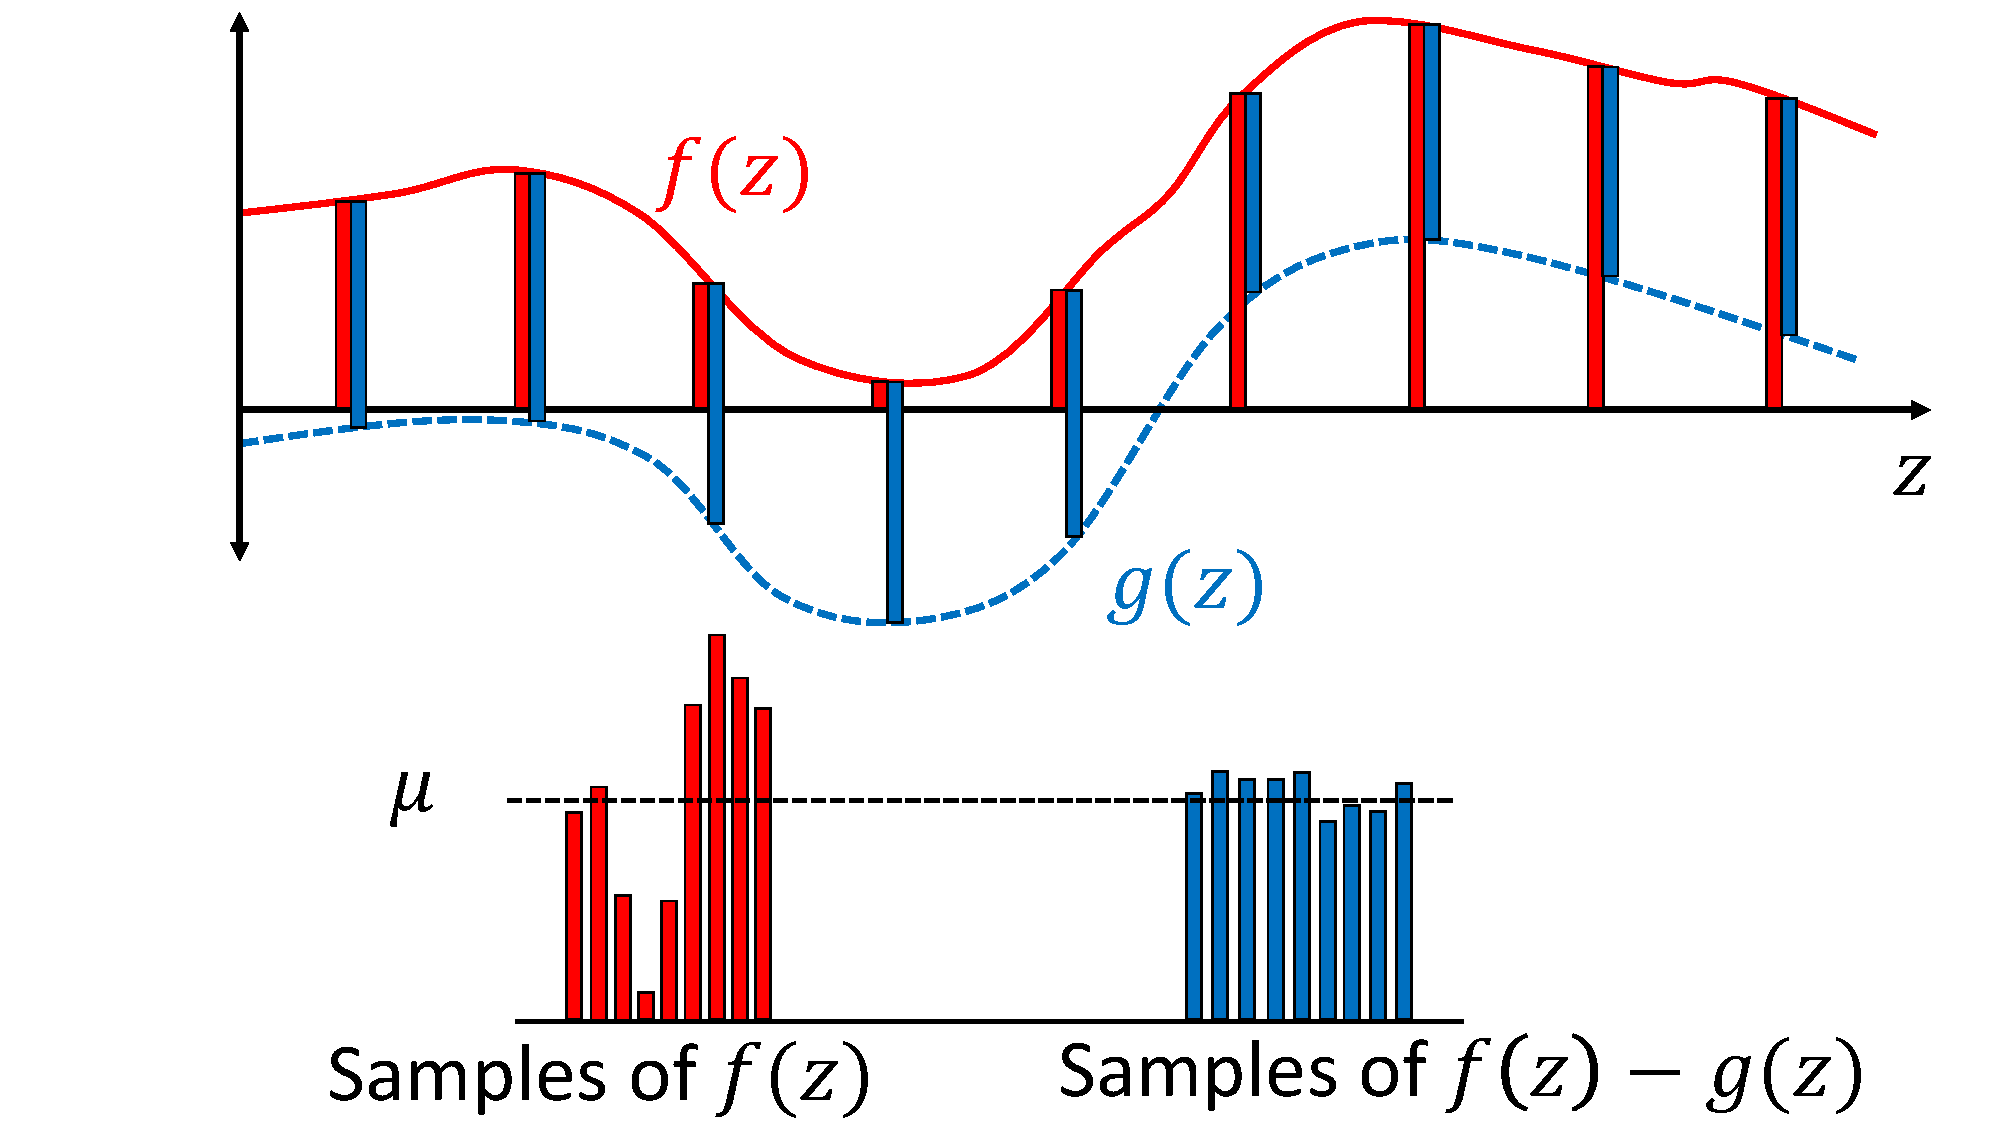
\includegraphics[width=\columnwidth]{figures/variance_reduction_extreme}
  \caption{\label{fig:variance_reduction}
  The samples from $f(z)$ have a higher variance than the samples
  from $f(z)-g(z)$ but the same mean. This is the key idea behind using control variates to reduce variance.}
\end{figure}

We can show that among all distributions with
fixed $\sigma^2_f$, $\sigma^2_a$, and $\alpha$ (equivalently $\rho$), this estimator is minimax optimal, i.e.\ it has the least variance among all unbiased estimators:

\begin{theorem}
\label{thm:main}
Among all unbiased
  estimators that are functions of $y^{(i)}$ and $g(z^{(i)})$, and for all distributions with a given $\sigma^2_f$, $\sigma^2_a$, and $\alpha$,
\begin{align}
  \label{eqn:varcontrol}
  \Var(\mucontrol) = \frac{1}{n} (\sigma^2_f (1 - \rho^2) + \sigma^2_a),
\end{align}
and no other estimator has a lower worst-case variance.
\end{theorem}

Comparing the variances of the two estimators (\refeqns{varsimple}{varcontrol}),
we define the \emph{data efficiency} as the ratio of the variances:
\begin{align}
\DE \eqdef \frac{\Var(\musimple)}{\Var(\mucontrol)} = \frac{1 + \gamma}{1-\rho^2 + \gamma},
\end{align}
where $\gamma \eqdef \sigma^2_a / \sigma^2_f$ is the normalized annotator variance.
Data efficiency is the key quantity in this paper:
  it is the multiplicative reduction in the number of samples required
  when using the control variates estimator $\mucontrol$ versus the sample mean $\musimple$.
Figure~\ref{fig:savings} shows the inverse data efficiency contours as a function of the correlation $\rho$
and $\gamma$.

\begin{figure}
\centering
  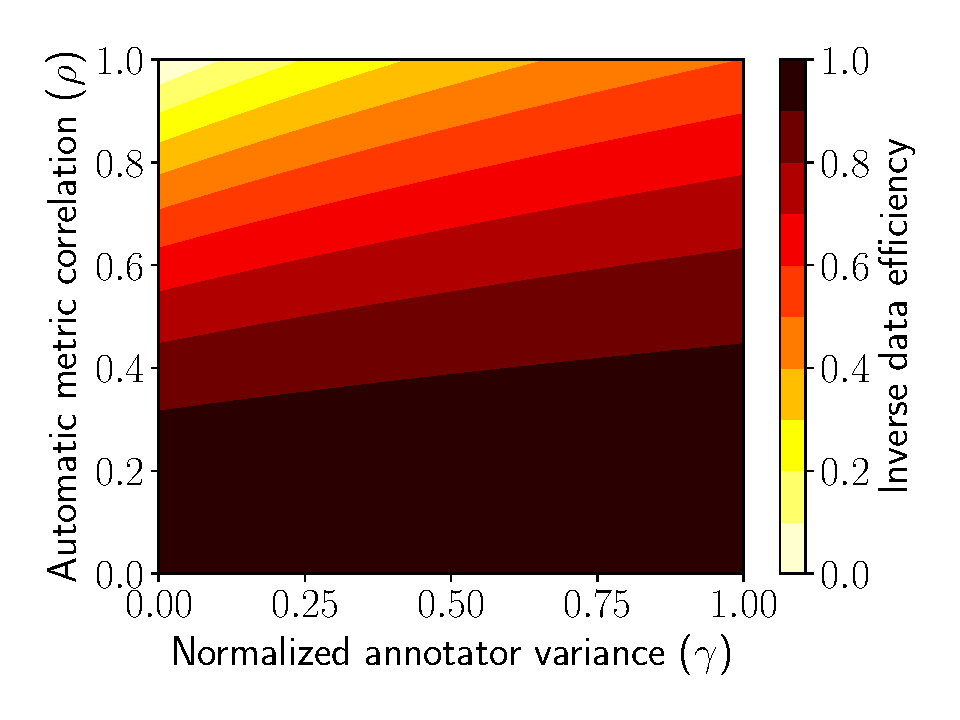
\includegraphics[width=\columnwidth]{figures/savings}
  \caption{\label{fig:savings} Inverse data efficiency for various values of
  $\gamma$ and $\rho$.  We need both low $\gamma$ and high $\rho$ to obtain
  significant gains.
  }
\end{figure}

When there is no correlation between human and automatic metrics ($\rho = 0$),
the data efficiency is naturally $1$ (no gain).
In order to achieve a data efficiency of
$2$ (half the labeling cost), we need $|\rho| \geq \sqrt{2}/2 \approx 0.707$.
Interestingly, even for an automatic metric with perfect correlation ($\rho=1$),
the data efficiency is still capped by $\frac{1 + \gamma}{\gamma}$:
unless $\gamma \to 0$ the data efficiency cannot increase unboundedly.
Intuitively, even
if we knew that $\rho=1$, $f(z)$ would be undetermined up to a
constant additive shift and just estimating the shift would incur a variance of $\frac{1}{n} \sigma_a^2$.




\subsection{Using the control variates estimator}
The control variates estimator can be easily integrated into an existing evaluation:
we run human evaluation on a random sample of system outputs, automatic evaluation on all the system outputs, and plug in these results into \refalg{estimate}.

It is vital that we are able to evaluate the automatic metric on a significantly larger set of examples than those with human evaluations to reliably normalize $g(z)$:
without these additional examples, it be can shown that the optimal minimax estimator for $\mu$ is simply the naive estimate $\musimple$.
Intuitively, this is because estimating the mean of $g(z)$ incurs an equally large variance as estimating $\mu$.
In other words, $g(z)$ is only useful if we have additional information about $g$ beyond the samples $\{z^{(i)}\}$.

\refalg{estimate} shows the estimator.
In practice, we do not know $\alpha = \Cov(f(z),g(z))$, so we use a plug-in estimate $\hat{\alpha}$ in line 3 to compute the estimate $\widetilde{\mu}$ in line 4.
We note that estimating $\alpha$ from data does introduce a $O(1/n)$ bias,
but when compared to the standard deviation which decays as $\Theta(1/\sqrt{n})$, this bias quickly goes to $0$.

\begin{proposition}
\label{prop:added_bias}
The estimator $\widetilde{\mu}$ in \refalg{estimate} has $O(1/n)$ bias.
\end{proposition}

\begin{algorithm}
      \caption{\label{alg:estimate}Control variates estimator}
      \begin{algorithmic}[1]
   \STATE{} {\bfseries Input:} $n$ human evaluations $y^{(i)}$ on system outputs $z^{(i)}$, \textit{normalized} automatic metric $g$ 
   \STATE{} $\overline{y} = \frac{1}{n} \sum_i y^{(i)}$
   \STATE{} $\hat{\alpha} = \frac{1}{n} \sum_i (y^{(i)} - \overline{y}) g(z^{(i)})$
   \STATE{} $\widetilde{\mu} = \frac{1}{n} \sum_i y^{(i)} - \hat{\alpha} g(z^{(i)})$
   \STATE{} {\bfseries return} $\widetilde{\mu}$
\end{algorithmic}
\end{algorithm}

An additional question that arises when applying \refalg{estimate} is figuring out how many samples $n$ to use.
Given a target variance, the number of samples can be estimated using \refeqn{varcontrol} with conservative estimates of $\sigma^2_f$, $\sigma^2_a$ and $\rho$.
Alternatively, our estimator can be combined with a dynamic stopping rule~\citep{mnih2008empirical} to stop data collection once we reach a target confidence interval.

\subsection{Discussion of assumptions}
We will soon see that empirical instantiations of $\gamma$ and $\rho$ lead to rather underwhelming data efficiencies in practice.
In light of our optimality result, does this mean there is no hope for gains?
Let us probe our assumptions.
We assumed that the human judgments are uncorrelated across different system outputs;
it is possible that a more accurate model of human annotators (e.g.\ \citet{passonneau2014benefits}) could offer improvements.
Perhaps with additional information about $g(z)$ such as calibrated confidence estimates,
we would be able to sample more adaptively.
Of course the most direct routes to improvement involve increasing the correlation of $g$ with human judgments and reducing annotator variance,
which we will discuss more later.




